\subsection{Standard Inverse Gamma Distribution}

The pdf of the inverse gamma is 

\begin{subequations}
\begin{align}
	\mathcal{IG}(x, \alpha, \lambda) &= \frac{\lambda^{\alpha}}{\Gamma(\alpha)} x^{-\alpha-1} \exp(-\frac{\lambda}{x}) \\
	&=\exp \frac{1}{x}\left[-\alpha\log(x) - \lambda/x + \alpha \log(\lambda) -\log\Gamma(\alpha)\right]
	\label{eq:pdf_inverse_gamma}
\end{align}
\end{subequations}

where $h(x) = \frac{1}{x}$, $\phi(x)=(\log(x), x), w= (-\alpha, -\lambda)$ and $Z(\alpha,\lambda) = \log\Gamma(\alpha) - \alpha\log\lambda$.

\subsubsection{Laplace Approximation of the standard inverse gamma distribution}

\begin{align*}
\text{log-pdf: } &(-\alpha-1)\log(x) - \lambda/x + \alpha \log(\lambda) -\log\Gamma(\alpha) \\
\text{1st derivative: }&  \frac{-\alpha-1}{x} + \frac{\lambda}{x^2}\\
\text{mode: }& \frac{-\alpha-1}{x} + \frac{\lambda}{x^2} = 0 \Leftrightarrow x = \frac{\lambda}{a+1}\\
\text{2nd derivative: }&  \frac{\alpha+1}{x^2} - 2\frac{\lambda}{x^3}\\
\text{insert mode: }& \frac{\alpha+1}{\frac{\lambda}{a+1}^2} - 2\frac{\lambda}{\frac{\lambda}{a+1}^3} = -\frac{(\alpha +1)^3}{\lambda^2} \\
\text{invert and times -1: }&\sigma^2 = \frac{\lambda^2}{(\alpha +1)^3}
\end{align*}

with $q(x) = \mathcal{N}(x; \mu = \frac{\lambda}{a+1}, \sigma^2 =\frac{\lambda^2}{(\alpha +1)^3} )$. 

\subsection{Log-Transform of the inverse Gamma distribution}

We transform the Inverse Gamma distribution with the log-transformation, i.e. $Y = \log(X)$. Therefore $g(x) = \log(x)$, and thereby $x(y) = g^{-1}(x) = \exp(y)$. It follows that the new pdf is 

\begin{subequations}
\begin{align}
	f_{Y\_\log}(y, \alpha, \lambda) &= \frac{\lambda^{\alpha}}{\Gamma(\alpha)} \exp(y)^{-\alpha-1} \exp(-\lambda/\exp(y)) \cdot \exp(y) \\
	&=  \frac{\lambda^{\alpha}}{\Gamma(\alpha)} \exp(y)^{-\alpha} \exp(-\lambda/\exp(y)) \\
	&= \exp\left[-\alpha x - \frac{\lambda}{\exp(x)} - \log\Gamma(\alpha) + \alpha\log(\lambda)\right]
	\label{eq:inv_gamma_trans_pdf}
\end{align}
\end{subequations}


with $h(y) = 1, \phi(y) = (y, \exp(y)), w=(-\alpha, \lambda)$ and $Z(\alpha, \lambda) = \log\Gamma(\alpha) - \alpha \log \lambda$.

\subsubsection{Laplace Approximation of the log-transformed Inverse Gamma Distribution}


\begin{align*}
\text{log-pdf: } &-\alpha y - \frac{\lambda}{\exp(y)} + C \\
\text{1st derivative: }&  -\alpha + \frac{\lambda}{\exp(y)}\\
\text{mode: }&  -\alpha + \frac{\lambda}{\exp(y)} = 0 \Leftrightarrow y = \log(\lambda/\alpha)\\
\text{2nd derivative: }&  -\frac{\lambda}{\exp(y)}\\
\text{insert mode: }&  -\frac{\lambda}{\exp(\log(\lambda/\alpha))} = -\alpha\\
\text{invert and times -1: }&\sigma^2 = \frac{1}{\alpha}
\end{align*}

\subsubsection{The Bridge for the log-transformed Inverse Gamma Distribution}

\begin{subequations}
\begin{align}
	\mu &= \log\left(\frac{\lambda}{\alpha}\right) \\
	\sigma^2 &= \frac{1}{\alpha} \\
	\alpha &= \frac{1}{\sigma^2}\\
	\lambda &= \frac{\exp(\mu)}{\sigma^2}
\end{align}
\end{subequations}

\begin{figure}[!htb]
	\centering
	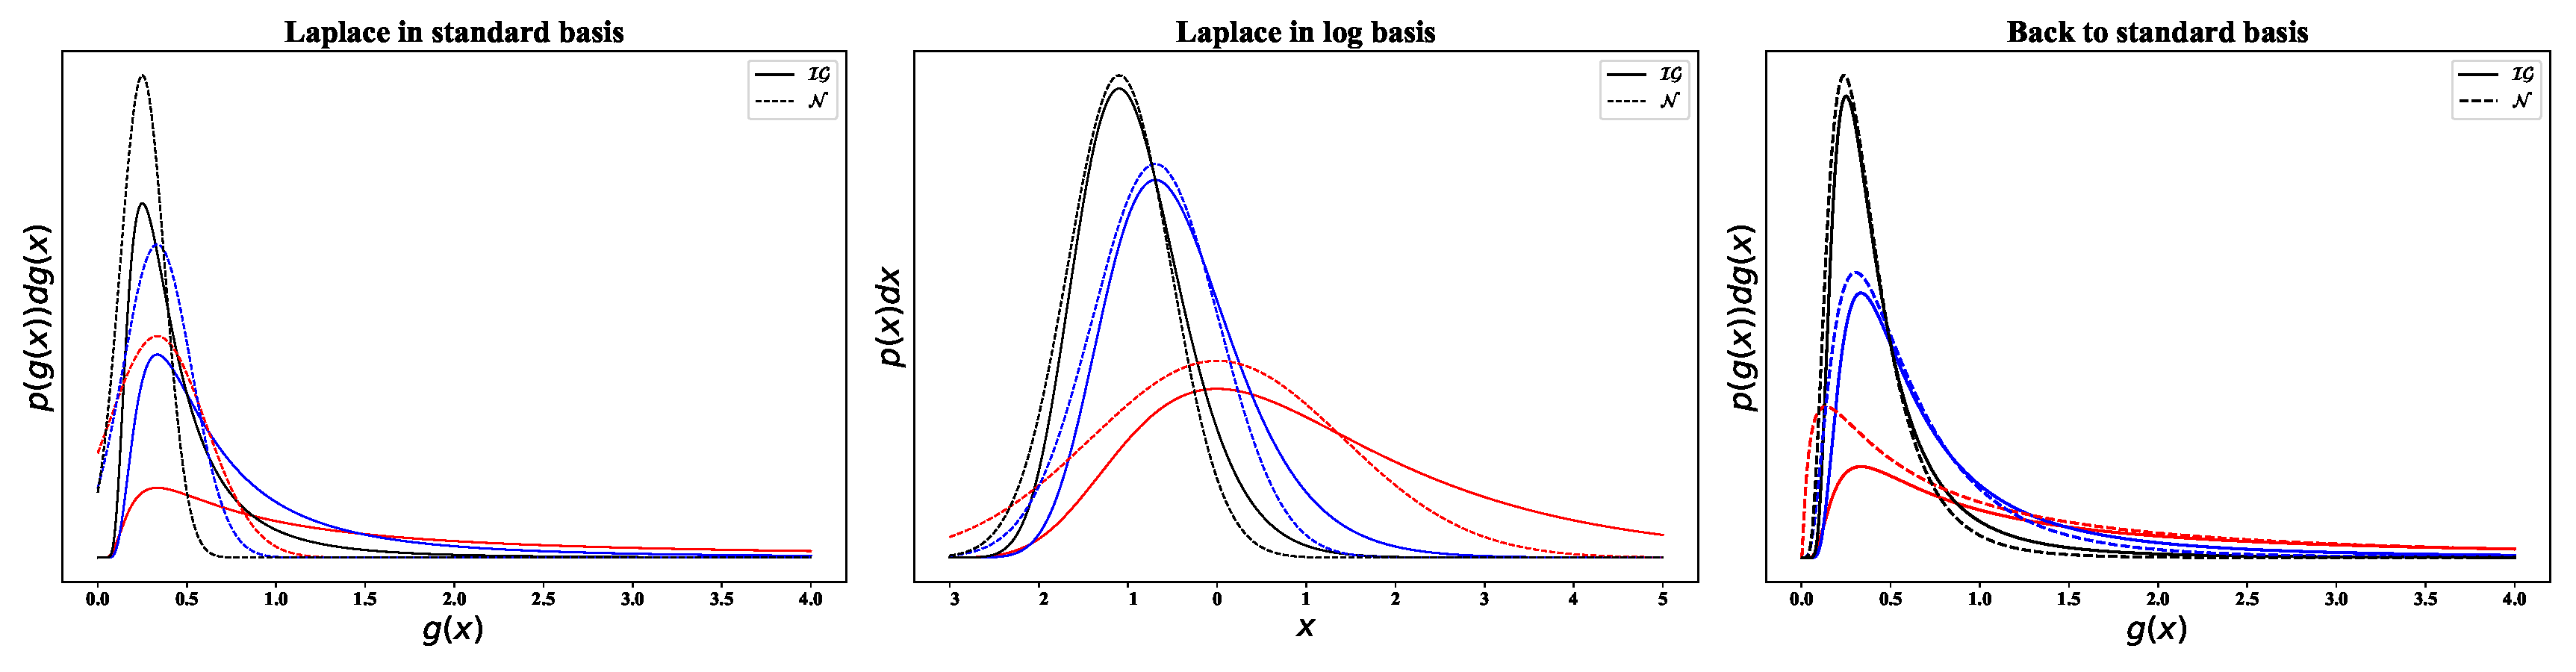
\includegraphics[width=\textwidth]{figures/inverse_gamma_log_bridge.pdf}
	\caption{inverse gamma log-bridge}
	\label{fig:inverse_gamma_log_bridge}
\end{figure}

\subsection{Sqrt-Transform of the inverse Gamma distribution}

We transform the Inverse Gamma distribution with the sqrt-transformation, i.e. $Y = \sqrt{X}$. Therefore $g(x) = \sqrt{x}$, and thereby $x(y) = g^{-1}(x) = y^2$. It follows that the new pdf is 

\begin{subequations}
\begin{align}
f_{Y\_\log}(y, \alpha, \lambda) &= \frac{\lambda^{\alpha}}{\Gamma(\alpha)} y^{2(-\alpha-1)} \exp(-\lambda/y^2)) \cdot 2y \\
&=  \frac{\lambda^{\alpha}}{\Gamma(\alpha)} y^{-2\alpha-\frac{1}{2}} \exp(-\lambda/y^2)) \\
&= \frac{1}{\sqrt{y}}\exp\left[-2\alpha \log(y) - \frac{\lambda}{y^2} - \log\Gamma(\alpha) + \alpha\log(\lambda)\right]
\label{eq:inv_gamma_sqrt_pdf}
\end{align}
\end{subequations}


with $h(y) = \frac{1}{\sqrt{y}}, \phi(y) = (\log(y), y^2), w=(-2\alpha, -\lambda)$ and $Z(\alpha, \lambda) = \log\Gamma(\alpha) - \alpha \log \lambda$.

\subsubsection{Laplace Approximation of the sqrt-transformed Inverse Gamma Distribution}

\begin{align*}
\text{log-pdf: } &(-2\alpha-1)\log(y) - \frac{\lambda}{y^2} + C \\
\text{1st derivative: }& -\frac{2\alpha+1}{y} + 2\frac{\lambda}{y^3} \\
\text{mode: }&  y = \sqrt{\frac{\alpha+0.5}{\lambda}}\\
\text{2nd derivative: }&  \frac{2\alpha+1}{y^2} - 6\frac{\lambda}{y^4}\\
\text{insert mode: }&  -4\frac{(\alpha+0.5)^2}{\lambda}\\
\text{invert and times -1: }&\sigma^2 = \frac{\lambda}{4 (\alpha+0.5)^2}
\end{align*}

yielding $q(y) = \mathcal{N}(y; \mu = \sqrt{\frac{\alpha+0.5}{\lambda}}, \sigma^2 = \frac{\lambda}{4 (\alpha+0.5)^2})$. 

\subsubsection{The Bridge for the sqrt-transformed Inverse Gamma Distribution}

\begin{subequations}
\begin{align}
\mu &= \sqrt\frac{\lambda}{\alpha} \\
\sigma^2 &= \frac{\lambda}{4\alpha^2} \\
\alpha &= \frac{\mu^2}{4\sigma^2}-0.5\\
\lambda &= \frac{\mu^4}{4\sigma^2}
\end{align}
\end{subequations}

\begin{figure}[!htb]
	\centering
	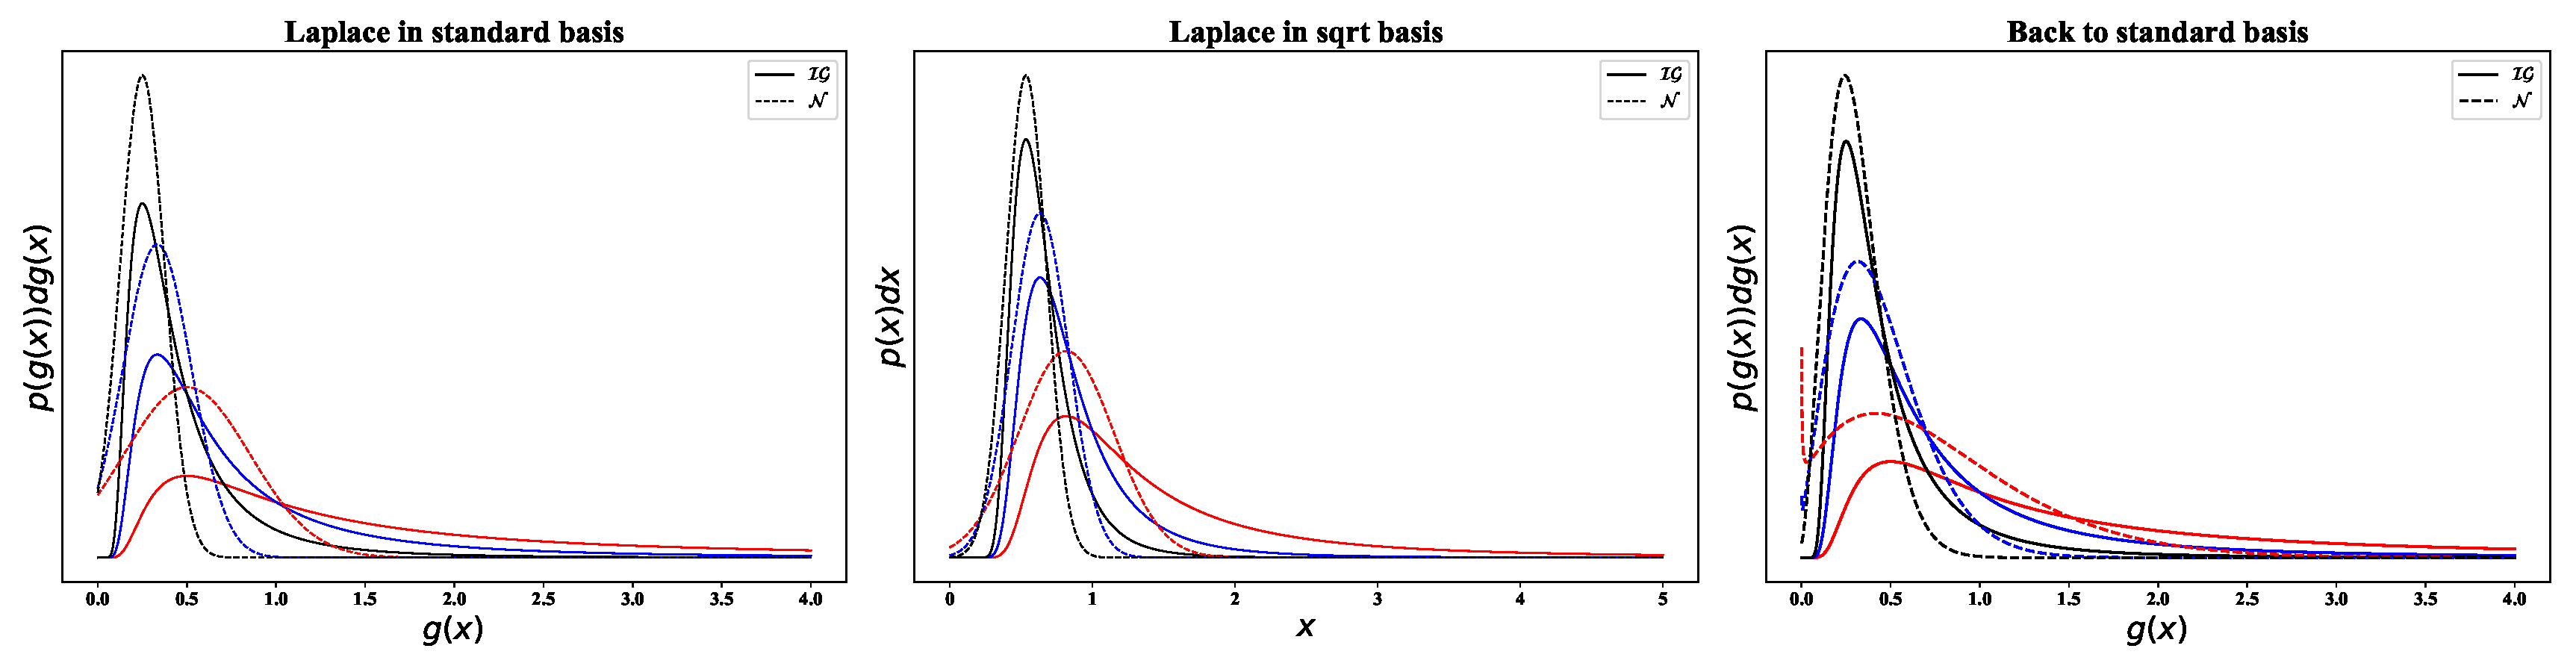
\includegraphics[width=\textwidth]{figures/inverse_gamma_sqrt_bridge.pdf}
	\caption{inverse gamma sqrt-bridge}
	\label{fig:inverse_gamma_sqrt_bridge}
\end{figure}